\subsection{Bouncy Castle Comparison}
\label{sec:performance_bouncycastle}

Bouncy Castle is an extensive suite of cryptography constructs, including those required for ECC. Bouncy Castle is originally a
Java library, but much of it has been ported to C\#.\cite{bouncycastle} Comparing OpenECC to Bouncy Castle will give an idea of the performance
compared to an alternative that is used in real-world applications.\footnote{The code performing the comparison and measurements
in Java can be found at \texttt{https://github.com/hypesystem/BouncyCastlePerformance}}

While much of Bouncy Castle has been ported to C\#, the Elliptic Curve ElGamal encryption has not. This makes it difficult to
give a realistic comparison of the two libraries, as only Elliptic Curve ElGamal, and no alternatives, is supported in OpenECC.

To get some idea of the relative running times, Bouncy Castle in Java is compared with OpenECC in C\#. A lot of the performance
difference may come down to differences between the virtual machines underlying the programs. As such, the constructs used in
Elliptic Curve ElGamal that have been ported to C\# (such as curve setup and key generation) have their running time measured
as well.

\begin{figure}[htb!]
	\centering
	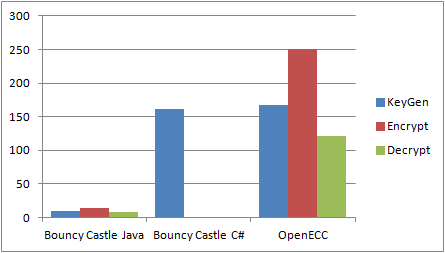
\includegraphics[width=0.9\textwidth]{performance/bouncycastle-comparison}
	\caption{Running time (ms) of Bouncy Castle in Java and C\# shown next to that of OpenECC. BouncyCastle C\# does not contain
		implementations of the encryption and decryption functions used, so these have not been measured.}
	\label{fig:bouncycastle-comparison-graph}
\end{figure}

We see a great difference between the two virtual machines: the key generation in Bouncy Castle's Java implementation takes
\(10 \text{ ms}\), whereas the Bouncy Castle C\# and OpenECC take \(161 \text{ ms}\) and \(168 \text{ ms}\), respectively.

Assuming that Bouncy Castle is implemented in the same way in both languages, the C\# implementation is \(16\) times slower
than the Java implementation. We can then project expected values for the encryption and decryption using EC ElGamal in Bouncy
Castle C\#: \(224 \text{ ms}\) and \(128 \text{ ms}\), respectively. These values leave the Bouncy Castle encryption \(26 \text{ ms}\)
faster than OpenECC, but the decryption \(7 \text{ ms}\) slower.

Bouncy Castle does not -- unlike OpenECC -- contain any encoding algorithm, which means that the testing has been slightly skewed.
The times measured for OpenECC contain encoding and decoding within the encryption and decryption steps. As seen in the component
analysis above, encoding accounts for \(6\%\) of the encryption time. Encryption without encoding takes \(235 \text{ms}\), leaving it
only \(11 \text{ ms}\) slower than the projected encryption runtime for Bouncy Castle C\#.

The OpenECC implementation compares well with Bouncy Castle C\#. The differences between the measurements in the virtual machines
can have many explanations, both to do with the internals of the virtual machines and the diagnostics tools used
(\texttt{System.Diagnostics.Stopwatch} in C\# and \texttt{System.nanoTime()} in Java).

The performance comparisons performed here show that the OpenECC implementation does have a performance that can be considered viable
compared to existing alternatives.\footnote{OpenECC should, however, not be used for real-world applications, see Appendix
\ref{app:disclaimer}.}